\subsection{Caso d'uso UC10: Compilazione questionari generati dinamicamente}
\begin{center}
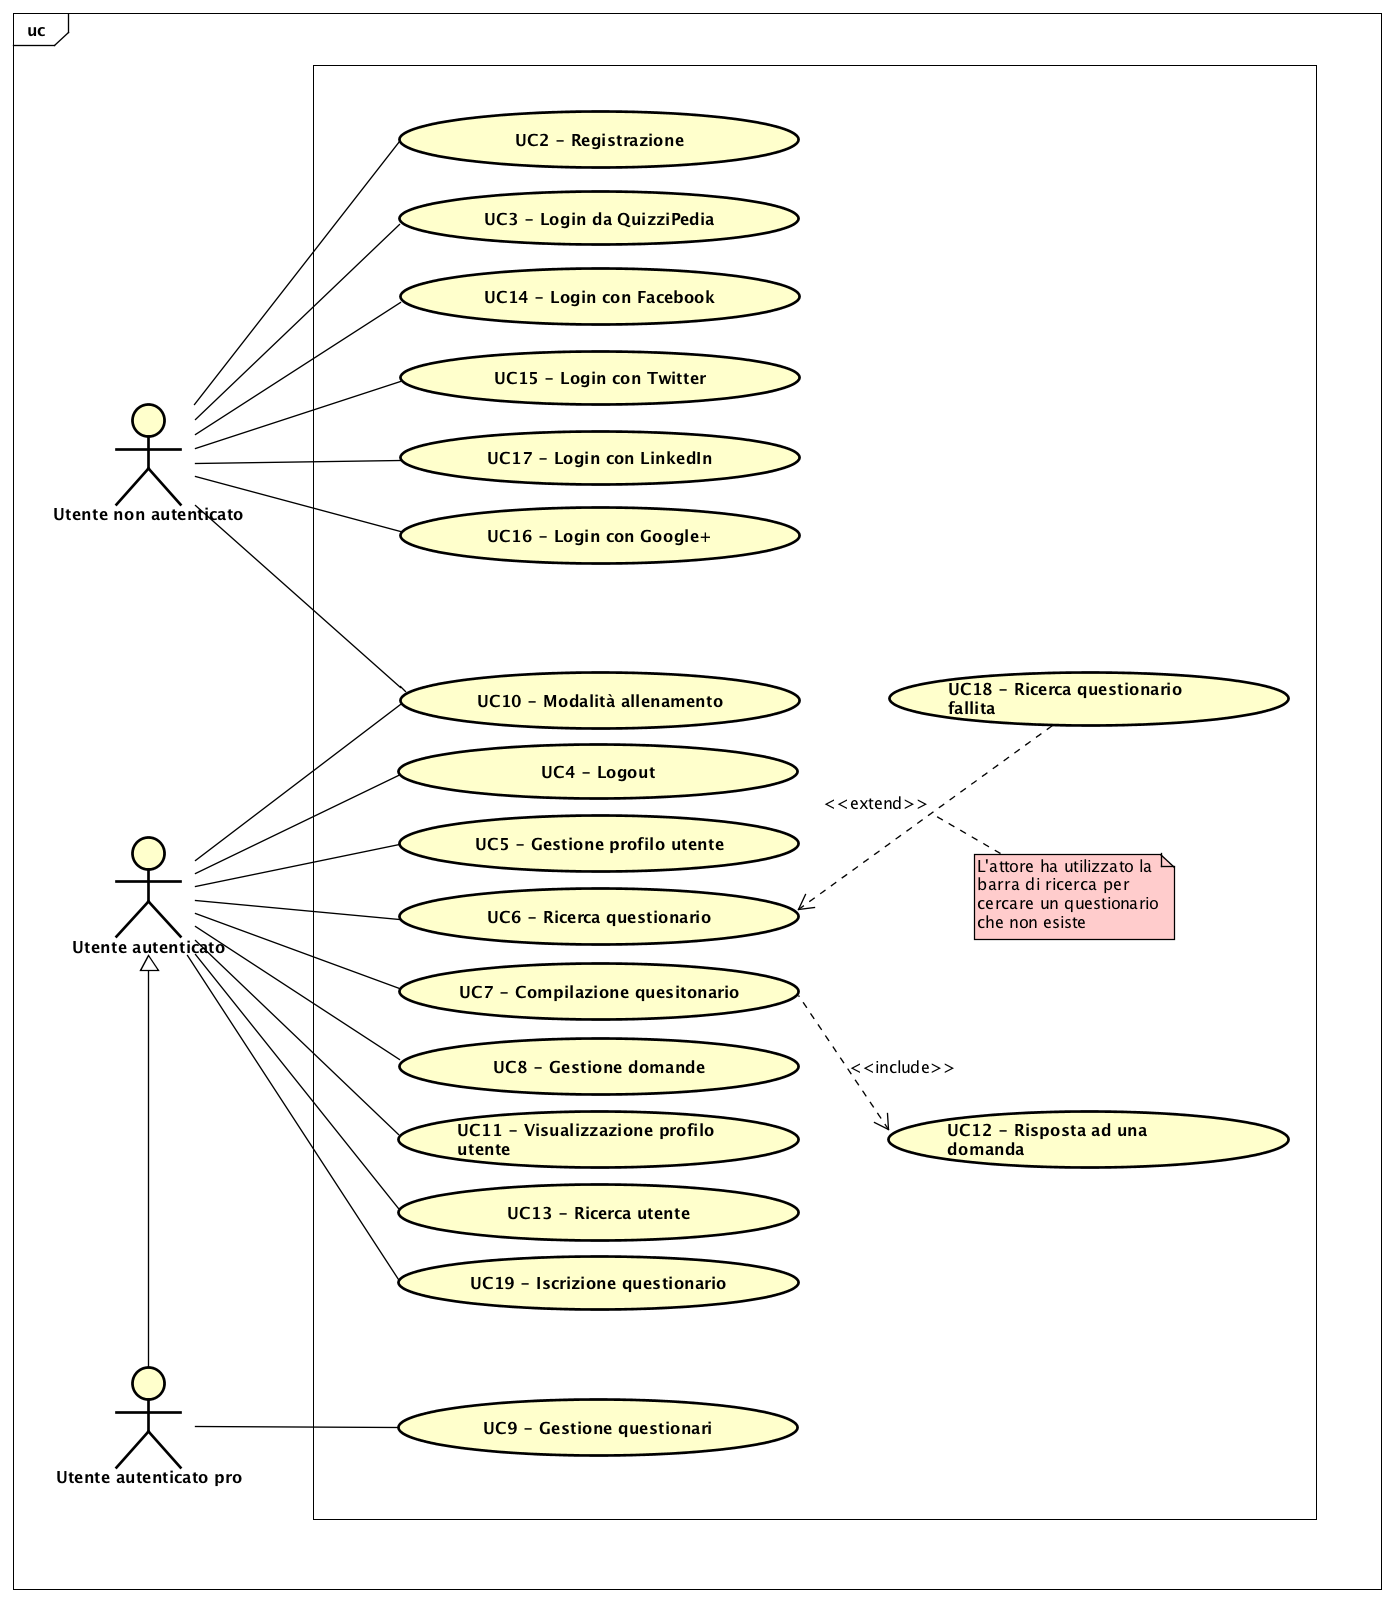
\includegraphics[scale=0.5]{UML/UC1.png}
\end{center}
\begin{itemize}
\item\textbf{Attori}: 
\item\textbf{Descrizione}: 
\item\textbf{Precondizione}: 
\item\textbf{Postcondizione}:
\item\textbf{Scenario principale}:
\end{itemize}